% TEMPLATE for Usenix papers, specifically to meet requirements of
%  USENIX '05
% originally a template for producing IEEE-format articles using LaTeX.
%   written by Matthew Ward, CS Department, Worcester Polytechnic Institute.
% adapted by David Beazley for his excellent SWIG paper in Proceedings,
%   Tcl 96
% turned into a smartass generic template by De Clarke, with thanks to
%   both the above pioneers
% use at your own risk.  Complaints to /dev/null.
% make it two column with no page numbering, default is 10 point

% Munged by Fred Douglis <douglis@research.att.com> 10/97 to separate
% the .sty file from the LaTeX source template, so that people can
% more easily include the .sty file into an existing document.  Also
% changed to more closely follow the style guidelines as represented
% by the Word sample file. 

% Note that since 2010, USENIX does not require endnotes. If you want
% foot of page notes, don't include the endnotes package in the 
% usepackage command, below.

% This version uses the latex2e styles, not the very ancient 2.09 stuff.
\documentclass[letterpaper,twocolumn,10pt]{article}
\usepackage{usenix,epsfig,endnotes}
\usepackage{subfigure}
\usepackage{color}
\usepackage{array}
\usepackage{longtable}
\usepackage{calc}
\usepackage{multirow}
\usepackage{hhline}
\usepackage{ifthen}
\begin{document}

%don't want date printed
\date{}

%make title bold and 14 pt font (Latex default is non-bold, 16 pt)
\title{\Large \bf Preserving Interactivity of GUI Applications}

%for single author (just remove % characters)
\author{
{\rm Hilfi Alkaff}\\
hilfialkaff@berkeley.edu
\and
{\rm Vu Chiem}\\
vuchiemh@berkeley.edu
\and
{\rm Andrew Wang}\\
awang@eecs.berkeley.edu
% copy the following lines to add more authors
% \and
% {\rm Name}\\
%Name Institution
} % end author

\maketitle

% Use the following at camera-ready time to suppress page numbers.
% Comment it out when you first submit the paper for review.
\thispagestyle{empty}


\subsection*{Abstract}
The manycore machines of the future will likely run a diverse set of concurrent workloads, placing additional demands on resource allocation and scheduling policies of the operating system to ensure interactive behavior of user applications while running high throughput batch processing jobs in the background. In our paper, we show that a degree of performance isolation can be achieved on Linux through the use of the existing CPUSET mechanism for realistic GUI applications.

\section{Introduction}

Motivation: existing schedulers do a poor job running simultaneous workloads with similar resource requirements and different interactive requirements. What we want is performance isolation.

Tessellation / Decomposition into the Cell model


More fascinating text. Features\endnote{Remember to use endnotes, not footnotes!} galore, plethora of promises.\\

\section{Related Work}

Things that should be mentioned here:
\begin{enumerate}
\item Linux schedulers: Redline, AIRS
\item mClock ?
\item fos, Barrelfish, Corey
\item Lithe: user level scheduler that is more hardware thread aware
\end{enumerate}

Some embedded literal typset code might 
look like the following :

{\tt \small
\begin{verbatim}
int wrap_fact(ClientData clientData,
              Tcl_Interp *interp,
              int argc, char *argv[]) {
    int result;
    int arg0;
    if (argc != 2) {
        interp->result = "wrong # args";
        return TCL_ERROR;
    }
    arg0 = atoi(argv[1]);
    result = fact(arg0);
    sprintf(interp->result,"%d",result);
    return TCL_OK;
}
\end{verbatim}
}

Now we're going to cite somebody.  Watch for the cite tag.
Here it comes~\cite{Chaum1981,Diffie1976}.  The tilde character (\~{})
in the source means a non-breaking space.  This way, your reference will
always be attached to the word that preceded it, instead of going to the
next line.

\section{Implementation}
\subsection{Channels}
We should mention these things in this section:
\begin{enumerate}
\item Lock free mechanism
\item Single consumer/producer
\item Loose measurement details (throughput for small message size)
\item Shared memory
\item Signalling mechanism
\end{enumerate}

Channel is the only communication mechanism that is being used in our system. The way we implement it is based on the existing 

\subsection{Nameserver} % This is could really be a subsubsection of channels
The nameserver functions similarly to a DNS server for channel IPC. It allows services to register themselves under an ASCII string {\tt name}, which can then be used in other applications and services. When a subsequent request is placed for this {\tt name}, the nameserver initializes a new channel and sends the shared memory ID to both processes. Further communication between the server and client happen without further nameserver intervention.

There is a slight chicken and egg problem here, since an application needs to already have a channel open to the nameserver before it can request channels to be opened. This is handled by reserving a globally known channel purely for this initialization step; applications will get a lock, inform the nameserver of its presence, wait for the nameserver to allocate a new channel for the two of them, and then unlock and continue communication on the new channel. Since this initialization channel is only used once by each process, there is little lock contention.

\subsection{Qt Embedded}
\begin{enumerate}
\item Framebuffer
\item Porting to tessellation
\item Client/server model
\item Decomposition
\end{enumerate}

\subsection{Resource Allocation Daemon}

Here's a typical figure reference.  The figure is centered at the
top of the column.  It's scaled.  It's explicitly placed.  You'll
have to tweak the numbers to get what you want.\\



This text came after the figure, so we'll casually refer to Figure 1
as we go on our merry way.


\section{Evaluation}

% you can also use the wonderful epsfig package...
\begin{figure*}[t]
  \begin{center}
    \subfigure[Sunspider JS benchmark]{\label{fig:edge-a}\includegraphics[scale=0.75]{sunspider.ps}}
    \subfigure[Textedit latency measurements]{\label{fig:edge-b}\includegraphics[scale=0.75]{textedit.ps}} \\
  \end{center}
  \label{fig:benchmarks}
\end{figure*}

\begin{table}[htp]
\caption{Textedit interactivity}
\label{textedit_table}
\begin{tabular}{|l | l | l | l |}
\hline
	&Latency ($\mu$s)	&Median	&Std dev\\ \hline
Qt, NL	&0.14	&0.13	&0.049\\
Qt, L	&30.60	&16.67	&37.24\\
Qt-C, NL	&0.16	&0.18	&0.033\\
Qt-C, L	&0.26	&0.15	&0.42\\
\hline
\end{tabular}
\end{table}

In this section, we examine how does our system perform on guaranteeing the promised resources even under tremendous load. Our experiments is run with Intel i7-880 2.93-GHz quad-core processors and inside the Qt virtual framebuffer. Load is simulated in our system by running 128 cpu-bound threads that runs an infinite loop.

<TABLE X> summarizes the latency of using our implementation of channels with varying message sizes. As we can see, the latency of sending a message from one point to another is very low.

To illustrate interactivity in our experiments, we use Qt sample textedit program and one of us will mash the keyboard and mouse for a couple of minutes and the latency between when the keyboard is pressed until when the change is reflected in the screen is measured. We also ensure that the events (i.e. keyboard or mouse pressed event) that are received in the server are all forwarded to the clients. Thus, our implementation is very reliable since it doesn't drop any of the registered events. 

As it can be seen in <GRAPH X>, our implementation loses to Qt performance-wise under no load. One speculation that we made to explain this difference is that we never use polling like the original Qt does and only use interrupts in our channel implementation. The overhead due to the frequent use of interrupts will be quite significant. 

With load running in the background the performance of our implementation almost does not change as promised by our guarantees, while the original implementation of Qt performs a lot worse. Finding out the work done by the background thread is outside the scope of this paper since what we are promising is that the GUI applications are able to run smoothly and not how much work is loss by the background threads. We expect the work done to be much lower in our case though, since we reserve a subset of our cores for our system services and the applications. 

The other measurement that we are evaluating our system on is by running a web browser, followed by SunSpider, a JavaScript benchmark. The result of this benchmark is similar as the previous one except that our implementation fares much better here.

\subsection{New Subsection}

It can get tricky typesetting Tcl and C code in LaTeX because they share
a lot of mystical feelings about certain magic characters.  You
will have to do a lot of escaping to typeset curly braces and percent
signs, for example, like this:
``The {\tt \%module} directive
sets the name of the initialization function.  This is optional, but is
recommended if building a Tcl 7.5 module.
Everything inside the {\tt \%\{, \%\}}
block is copied directly into the output. allowing the inclusion of
header files and additional C code." \\

Sometimes you want to really call attention to a piece of text.  You
can center it in the column like this:
\begin{center}
{\tt \_1008e614\_Vector\_p}
\end{center}
and people will really notice it.\\

\noindent
The noindent at the start of this paragraph makes it clear that it's
a continuation of the preceding text, not a new para in its own right.


Now this is an ingenious way to get a forced space.
{\tt Real~$*$} and {\tt double~$*$} are equivalent. 

Now here is another way to call attention to a line of code, but instead
of centering it, we noindent and bold it.\\

\noindent
{\bf \tt size\_t : fread ptr size nobj stream } \\

And here we have made an indented para like a definition tag (dt)
in HTML.  You don't need a surrounding list macro pair.
\begin{itemize}
\item[]  {\tt fread} reads from {\tt stream} into the array {\tt ptr} at
most {\tt nobj} objects of size {\tt size}.   {\tt fread} returns
the number of objects read. 
\end{itemize}
This concludes the definitions tag.

\subsection{How to Build Your Paper}

You have to run {\tt latex} once to prepare your references for
munging.  Then run {\tt bibtex} to build your bibliography metadata.
Then run {\tt latex} twice to ensure all references have been resolved.
If your source file is called {\tt usenixTemplate.tex} and your {\tt
  bibtex} file is called {\tt usenixTemplate.bib}, here's what you do:
{\tt \small
\begin{verbatim}
latex usenixTemplate
bibtex usenixTemplate
latex usenixTemplate
latex usenixTemplate
\end{verbatim}
}


\subsection{Last SubSection}

Well, it's getting boring isn't it.  This is the last subsection
before we wrap it up.

\section{Acknowledgments}

A polite author always includes acknowledgments.  Thank everyone,
especially those who funded the work. 

\section{Availability}

It's great when this section says that MyWonderfulApp is free software, 
available via anonymous FTP from

\begin{center}
{\tt ftp.site.dom/pub/myname/Wonderful}\\
\end{center}

Also, it's even greater when you can write that information is also 
available on the Wonderful homepage at 

\begin{center}
{\tt http://www.site.dom/\~{}myname/SWIG}
\end{center}

Now we get serious and fill in those references.  Remember you will
have to run latex twice on the document in order to resolve those
cite tags you met earlier.  This is where they get resolved.
We've preserved some real ones in addition to the template-speak.
After the bibliography you are DONE.

\footnotesize{\bibliographystyle{acm}
\bibliography{bibliography}}

\theendnotes

\end{document}







